\section{Question 4}\label{sec:q4}    

In the field of astrodynamics, there are a number of concepts and definitions to describe the position of points on Earth as well as celestial objects.

\subsection{4a}
\textit{To describe the position of points on the surface of the Earth, the following concepts are used: equatorial plane, meridian, geographic longitude, geocentric latitude, standard ellipsoid, geodetic latitude. Provide an accurate description of these concepts.} \\
The equatorial plate is the plane perpendicular to the rotation axis of the earth, in the middle between the North pole and the South pole:
\begin{figure}[H]
    \centering
    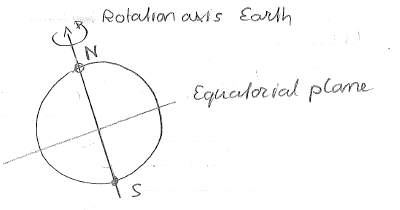
\includegraphics[width=0.6\columnwidth]{Figures/4a1.png}
    \caption{Equatorial plane}
    \label{fig:4a1}
\end{figure}

The meridian is a circle around the earth that goes through the South pole and North pole.
\begin{figure}[H]
    \centering
    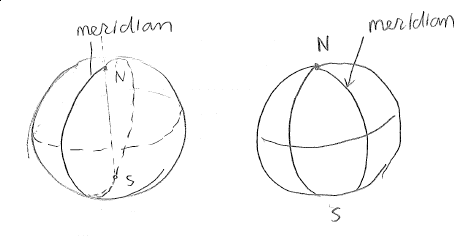
\includegraphics[width=0.6\columnwidth]{Figures/4a2.png}
    \caption{Meridian}
    \label{fig:4a2}
\end{figure}

Geographic longitude axis is the angle along the equatorial between the Greenwich meridian and the meridian of the observer w.r.t. to the centre of the Earth.
\begin{figure}[H]
    \centering
    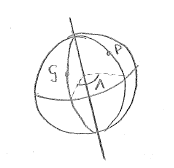
\includegraphics[width=0.3\columnwidth]{Figures/4a3.png}
    \caption{Equatorial plane}
    \label{fig:4a3}
\end{figure}

The geocentric latitude $\phi$ is the angle along the meridian of the observer from the equatorial plane to the observer w.r.t. to the centre of the Earth.
\begin{figure}[H]
    \centering
    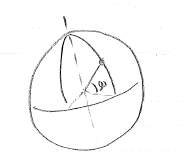
\includegraphics[width=0.3\columnwidth]{Figures/4a4.png}
    \caption{Equatorial plane}
    \label{fig:4a4}
\end{figure}

The standard ellipsoid is the ellipse that approximates the true shape of the Earth, by taking into account the Earth's flattening. \\

The geodetic latitude is to the standard ellipsoid what the geocentric latitude is to a circular meridian. It is the angle from the equatorial plane to the observer, along this standard ellipsoid.\\

\subsection{4b}
\textit{To describe the position of celestial objects, the following concepts are used: celestial sphere, celestial equator, hour circle, declination, right ascending node, ecliptic, obliquity of the ecliptic, vernal equinox. Provide an accurate description of these concepts.} \\

The \textbf{celestial sphere} is a fictitious sphere on which the sky, as seen from a planet, is projected. It defines a coordinate system XYZ, for which the Z-direction is the celestial North pole, and the X-direction points towards the constellation of Aries. \\
The \textbf{celestial equator} is the intersection of Earth's equatorial plane and the celestial sphere.
\textbf{Hour circle} are similar to meridians, but roughly divide up the Earth into 24 equal parts. The angle between two hour lines corresponds to one hour of Earth's rotation.\\
\textbf{Right ascending node} is the horizontal angle between the direction of the vernal equinox and a point on the celestial sphere. This angle is defined parallel to the celestial equator. \\
\textbf{Declination} is the vertical counterpart to the right ascending node. It is the vertical angle between the celestial equator plane and a point on the celestial sphere.\\
The \textbf{ecliptic} is the path of the Sun over the celestial sphere.\\
\textbf{Obliquity of the ecliptic} is the angle $\epsilon$, which is the angle between the equatorial plane and the ecliptic plane.\\
\textbf{Vernal equinox} is the point in Earth's movement around the sun where Earths rotational axis is perpendicular to the Earth-Sun line. This is also the points of intersection of the celestial equator and the ecliptic. The vernal equinox is the moment where it moves from the Southern hemisphere of the Earth to the Northern hemisphere of the Earth (which marks the start of spring on the Northern hemisphere).\\


\subsection{4c}
\textit{Explain why the vernal equinox is not a fixed point on the celestial sphere, but moves along it. Is the amplitude of luni-solar precession $12^\circ$, $23^\circ$ or $34^\circ$? Is the amplitude of the luni-solar nutation $9^\circ$, $9'$ or $9''$? Do the luni-solar precession and planetary precession influence the obliquity of the ecliptic?} \\
The vernal equinox moves constantly along the celestial sphere, because the celestial sphere and the ecliptic are continuously in motion. \\
The amplitude of luni-solar precession is about $23^\circ$. \\
The amplitude of luni-solar nutation is about 9''. \\
The luni-solar precession and planetary precession do not influence the obliquity of the ecliptic, but it does "spin" the Earth's equator around the ecliptic North pole. \\



\subsection{4d}
\textit{To define time, the following concepts are used: sidereal time, solar time, mean solar time, universal time (UT), atomic time (TAI), and universal time coordinated (UTC). Provide an accurate description of these concepts.} \\

From slides:\\
\textbf{Sidereal time} is time defined by the angular distance covered by the vernal equinox on the celestial sphere after its last crossing of the observer’s celestial meridian.\\
\textbf{Solar time} is time defined by the angular distance covered by the Sun on the celestial sphere after its last crossing of the observer’s celestial meridian.\\
\textbf{Mean solar time} is defined as the hour angle of the mean Sun plus 12 hr.\\
\textbf{Universal time} is today’s realization of a mean solar time, derived from GMST by a conventional relation.\\
A standardized mean solar time, based on a fictitious, mean Sun that moves at a uniform rate eastward along the celestial equator.\\
\textbf{Atomic time} is time based on the analysis of about 200 frequency standards (atomic clocks) maintained by several countries to keep a unit of time as close to the ideal SI second as possible (defined in terms of Cesium 133 transitions).\\
\textbf{Universal time coordinated} is a hybrid standard of time, of which the progression is determined by atomic time (TAI), but leap seconds are introduced, when needed, to keep up with Universal Time (UT1).
